\section{Adaptation electronics simulation}
\label{sec:elec}
Here we  consider the adaptation  electronics starting from  the power
detection up  to the analog to  digital conversion and  the final data
see fig.~\ref{fig:detscheme}.  In this chain, the main components are:
the power detector, the adaptation  board, the SD front end filter and
the ADC.   Some other  minor elements (minor  in the sense  they won't
modify the  signal shape or SNR  but only its  amplitude, like cables,
75-50 adapter or other lossy element) won't be simulated.
\subsection{power detection}
The step of the power detection is the most specific to EASIER system.
We present  here three methods  to simulate the power  detector.  They
are  closely related,  two of  them are  based on  a convolution  in a
simular way  I had done in  my thesis. The  third one is based  on the
frequency response.  To  test the methods we have  calibration data we
had taken  back in 2013.  The setup is  composed of a  C-band antennna
followed by a  power detector.  The signal is  recorded with the large
bandwidth oscilloscope simultaneously after  the antenna and the after
the  power   detector.   We  have  data  with   only  backgroud  noise
(fig.~\ref{fig:signalexample} left) and data with short pulses emitted
with an electronic lighter (fig.~\ref{fig:signalexample} right).
\begin{figure}[!ht]
  \centering
  \hspace*{-3ex}
  \subfigure{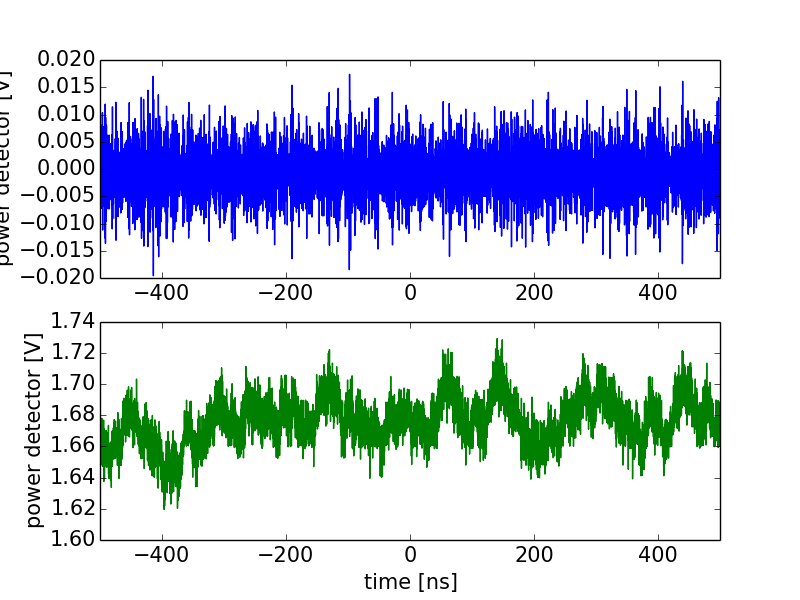
\includegraphics[width=0.49\linewidth]{noiseRFPD.png}}
  \subfigure{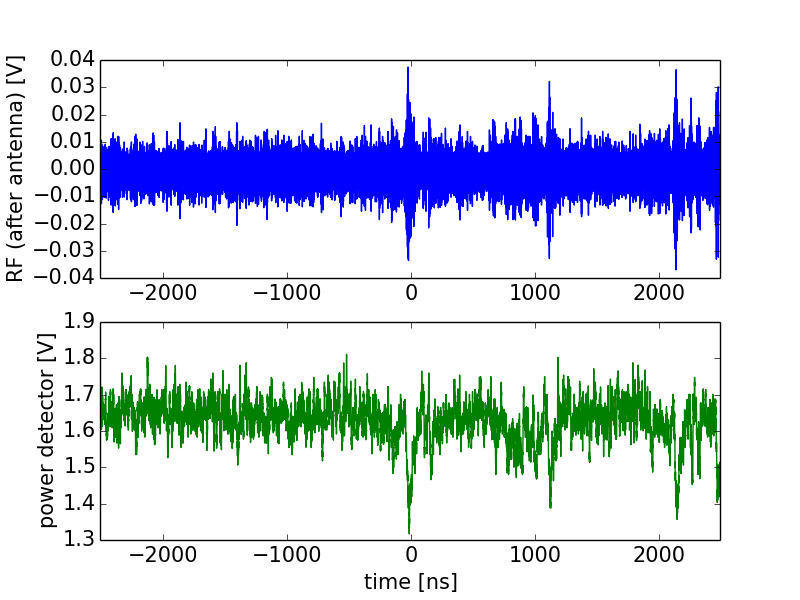
\includegraphics[width=0.49\linewidth]{signalexample.png}}
  \caption{example of calibration data, with only background noise (left), and with pulses (right)}
  \label{fig:signalexample}
\end{figure}

\subsubsection{DC calibration}
We first look at the calibration  of the DC component. We will use the
noise data to determine it. The method is very simple we just plot the
average  of the  power detector  waveform  against the  RF average  in
dBm. The  only interesting detail  here is the difference  between the
average of the log ($\rm <P> = \frac{1}{N}\Sigma P_{dBm}$) and the log
of the  average ($\rm <P>  = \frac{10}{N} \log_10 \Sigma  P_{mW}$). We
see these  characteristics on the  figure~\ref{fig:pdcarac}.  The main
difference  is   the  offset,  the   slope  found  from  the   fit  is
approximately the same.
\begin{figure}[!ht]
  \centering
  \hspace*{-3ex}
  \subfigure{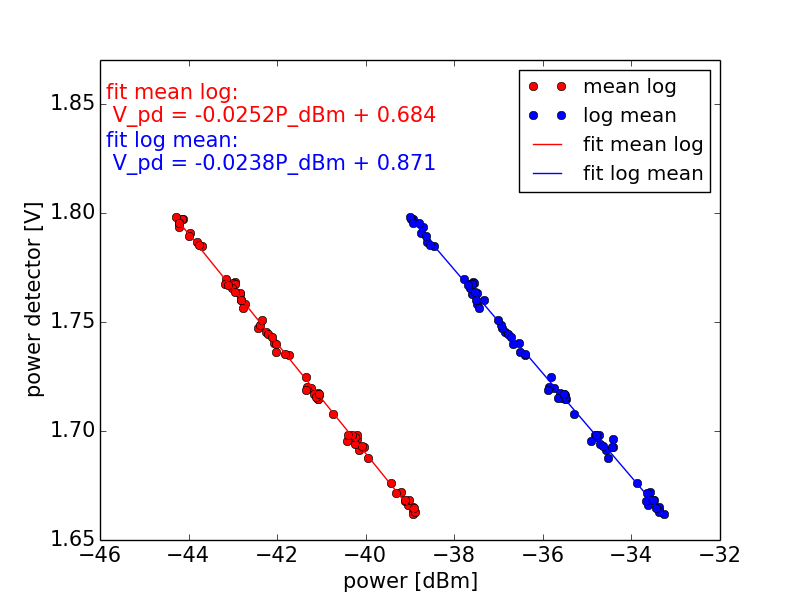
\includegraphics[width=0.60\linewidth]{powerdetDCcarac.png}}
  \caption{caracteristics of the power detector in the case we take the log of the mean power or in the case we take the mean of the log power}
  \label{fig:pdcarac}
\end{figure}
This  characteristics is  only  valid to  relate  the baseline  value,
i.e. mean values. If we want  to reproduce the waveform, we need a bit
more  complicated methods. We  present some  example in  the following
paragraphs.

\subsubsection{convolution with floating parameters (method 1)}
We  found  that a  good  way  to simulate  the  power  detector is  by
performing  a convolution  of the  signal in  dBm with  an exponential
decay function.   \\ We  want to reproduce  the power  detector signal
from the RF signal. Here are the steps we follow:
\begin{itemize}
\item transform RF signal in dBm
\item do the convolution with $f(t) = A\cdot \exp{\frac{t}{\tau}}$
\item  transform linearly  the  result to  obtain  the power  detector
  waveform: $V_{sim} = a\cdot V_{conv} + b$
\end{itemize}
In order to  find the parameters $\tau$,  a and b, we scan  a range of
values of  $\tau$, and then  fit $V_{conv}$ versus $V_{PD}$.   Then we
search for $\tau$, a and b  that minimize the distance $\rm d = \Sigma
(V_{sim} -  V_{PD})^2$ between the  two waveforms.  This  procedure is
perfomed on  20 waveforms  and the average  parameters are  chosen (cf
table~\ref{tab:method1tab}).
\begin{table}[h!]
  \centering
  \caption{parameters for the power detection}
  \label{tab:method1tab}
  \begin{tabular}{|c||c|c|c|}
    \hline
    & $\tau$ [ns] & a & b \\
    \hline
    with capacitor & $\rm 4.7 \pm 0.2$ & $\rm -0.019 \pm 0.001 $ & $\rm 0.88 \pm 0.04 $ \\
    \hline
    without capacitor & $\rm 35.2 \pm 2.2$ & $\rm -0.022 \pm 0.001 $  & $\rm 0.79 \pm 0.04 $\\
    \hline
  \end{tabular}
\end{table}
An example of a resulting simulated signal overlayed with the original
one is shown in the fig.~\ref{fig:m1ex} (middle) and the difference is
shown in the fig.~\ref{fig:m1ex} (bottom).
\begin{figure}[!ht]
  \centering
  \hspace*{-3ex}
  \subfigure{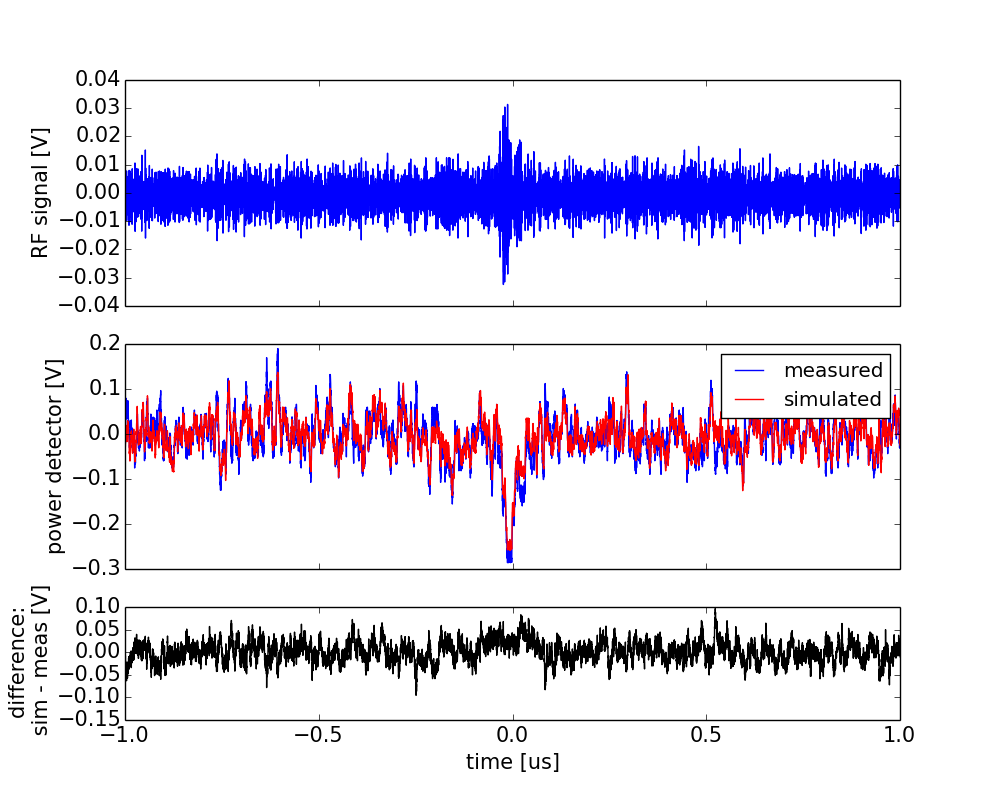
\includegraphics[width=0.49\linewidth]{nocapa_method1.png}}
  \subfigure{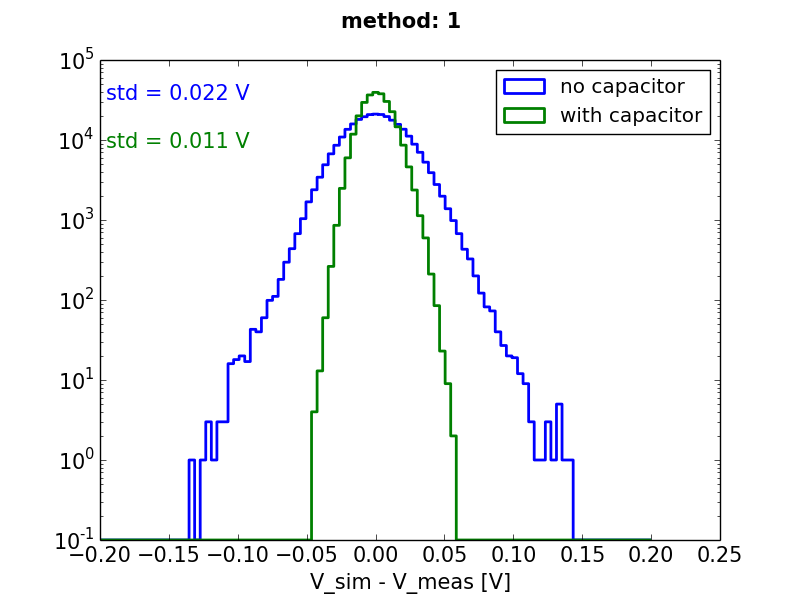
\includegraphics[width=0.49\linewidth]{res_method1.png}}
  \caption{top:  RF  waveform,  middle:  power detector  measured  and
    simulated, bottom: difference}
  \label{fig:m1ex}
\end{figure}
When  using the  average parameters  to all  waveforms, we  obtain the
residuals distribution in the figure~\ref{fig:m1ex}. The standard
deviation  for  the  no  capacitor  case  is 22mV  and  11mV  for  the
capacitor.

\newpage
\subsubsection{transfer function method}
Another way  to simulate  the power detector  response can be  done by
looking at the transfer function  in the frequency domain. This can be
seen  as a  filter  response.  In  practice,  we need  to  use the  DC
caracteristics we  already found (cf  fig.~\ref{fig:pdcarac}) and then
look  at the frequency  spectrum of  the signal  before and  after the
power detector.  Note that the  RF signal is first transformed in dBm,
i.e. in logarithmic  scale. We use the waveforms  presented before for
the convolution method.  On  the figures~\ref{fig:pdspec1} we show the
spectra  before  and  after  the  power  detector  (left),  the  ratio
(middle),     an      example     of     the      phase     difference
(right). Fig.~\ref{fig:pdspec1} is the  case when the capacitor is used
and fig.~\ref{fig:pdspec2} is  the no  capacitor  case. We  see that  the
capacitor case filters at lower frequencies as expected.
\begin{figure}[!ht]
  \centering
  \hspace*{-3ex}
  \subfigure{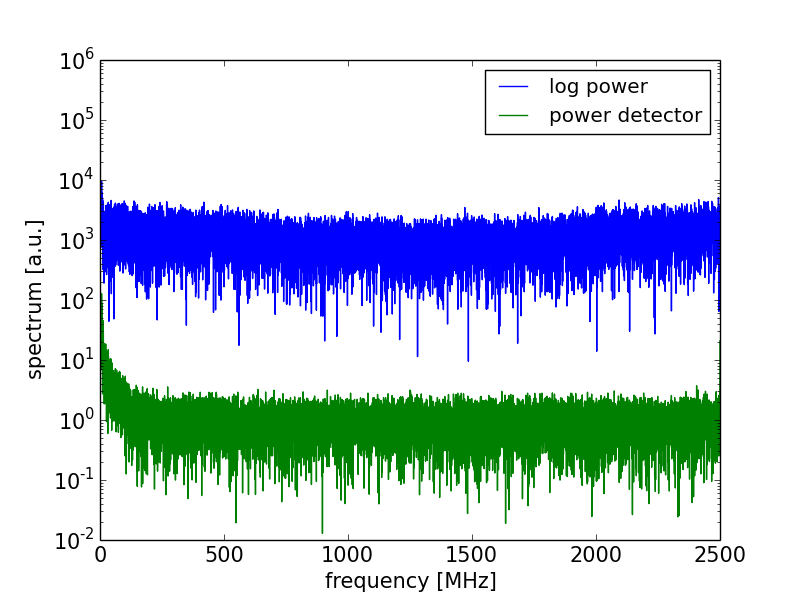
\includegraphics[width=0.32\linewidth]{c_spec.png}}
  \subfigure{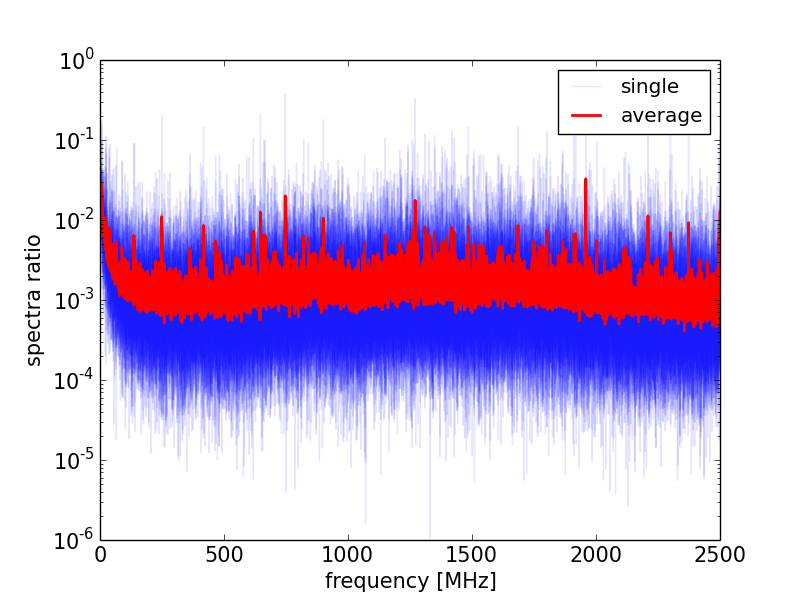
\includegraphics[width=0.32\linewidth]{c_ratio.png}}
  \subfigure{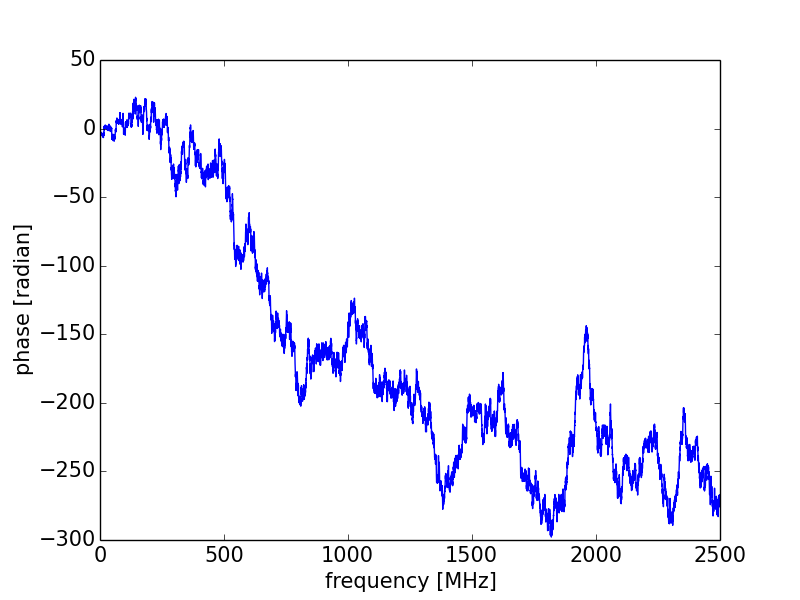
\includegraphics[width=0.32\linewidth]{c_phase.png}}
  \caption{capacitor case (left: spectrum, middle: ratio after/before, right: phase difference)}
  \label{fig:pdspec1}
\end{figure}

\begin{figure}[!ht]
  \centering
  \hspace*{-3ex}
  \subfigure{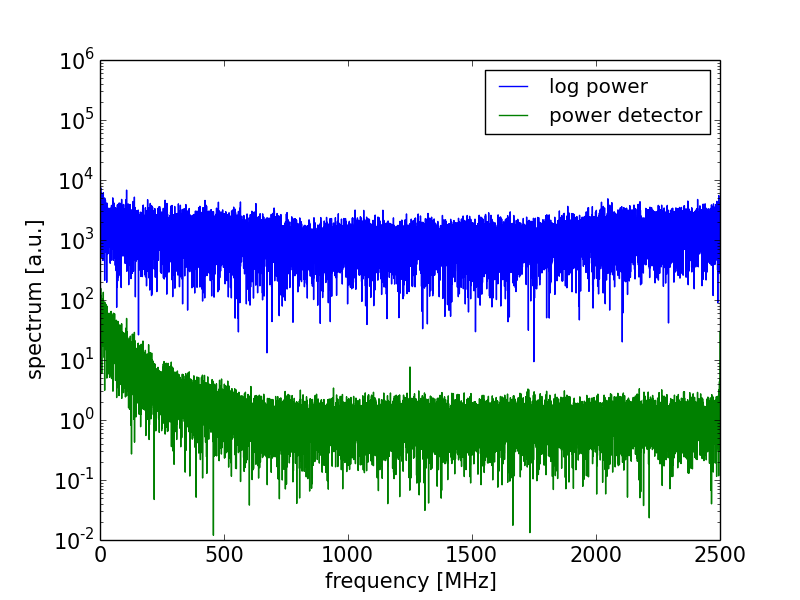
\includegraphics[width=0.32\linewidth]{nc_spec.png}}
  \subfigure{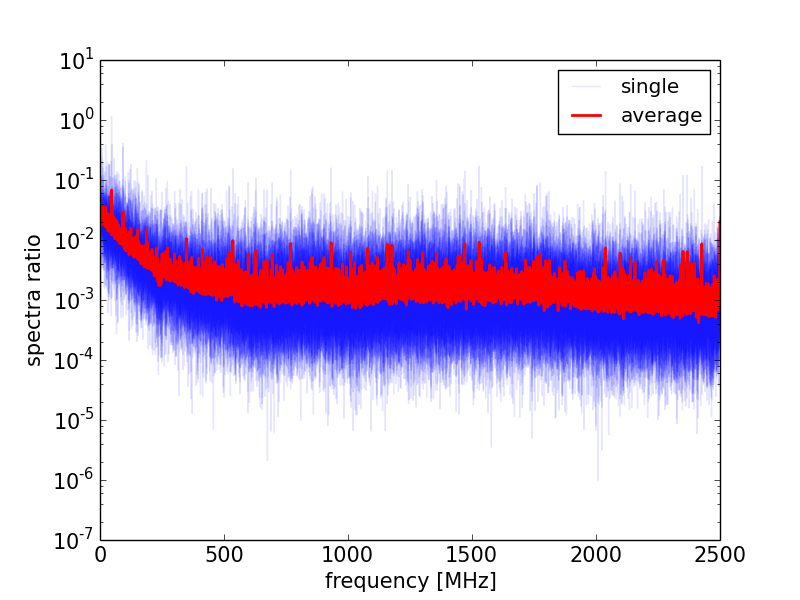
\includegraphics[width=0.32\linewidth]{nc_ratio.png}}
  \subfigure{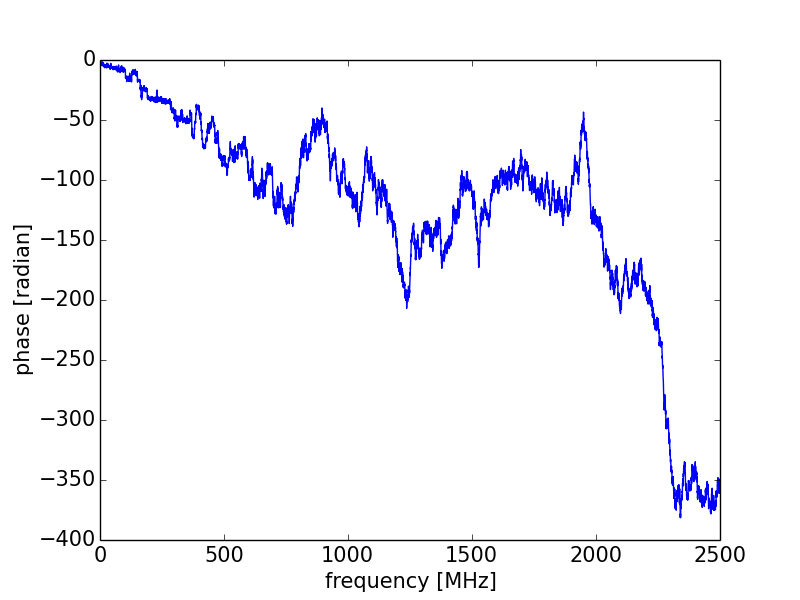
\includegraphics[width=0.32\linewidth]{nc_phase.png}}
  \caption{no capacitor case (left: spectrum, middle: ratio after/before, right: phase difference)}
  \label{fig:pdspec2}
\end{figure}
We  show an  example of  waveform for  the no  capacitor case  and the
distribution of  the difference  in the fig.~\ref{fig:m2ex}.  For this
method, the residuals are larger than for the first method.

\begin{figure}[!ht]
  \centering
  \hspace*{-3ex}
  \subfigure{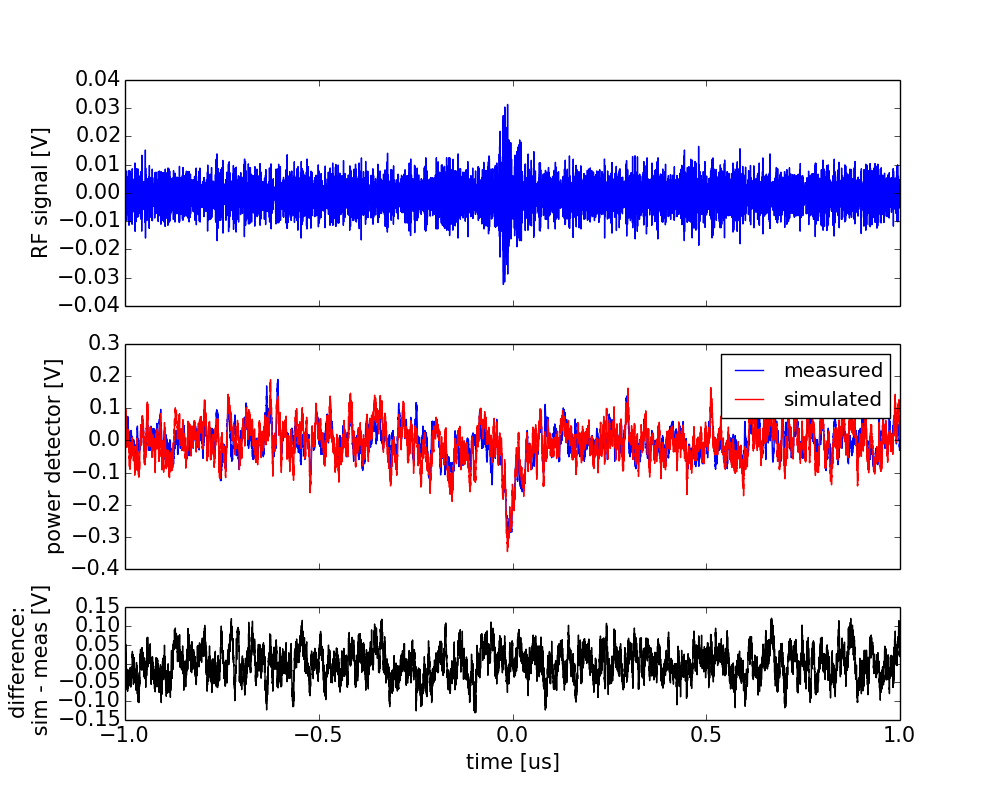
\includegraphics[width=0.49\linewidth]{nocapa_method2.png}}
  \subfigure{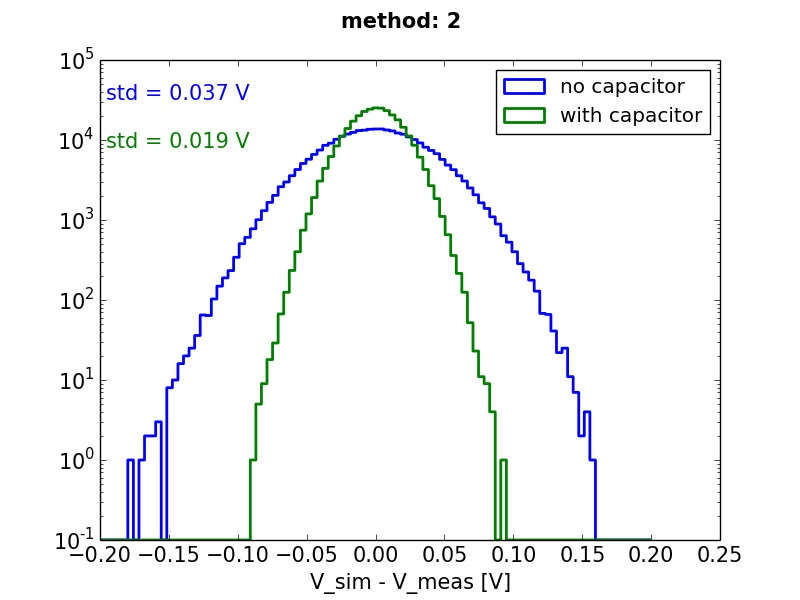
\includegraphics[width=0.49\linewidth]{res_method2.png}}
%  \subfigure{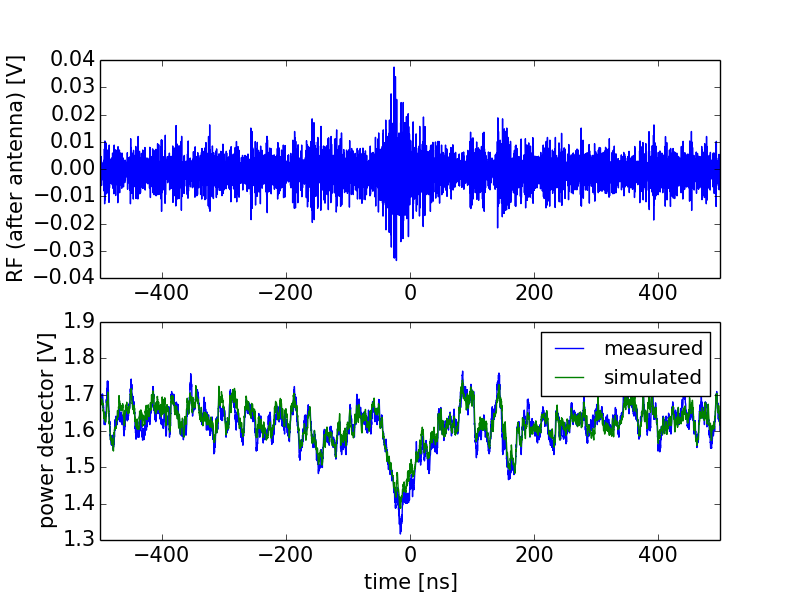
\includegraphics[width=0.49\linewidth]{examplepowerdetsim.png}}
%  \subfigure{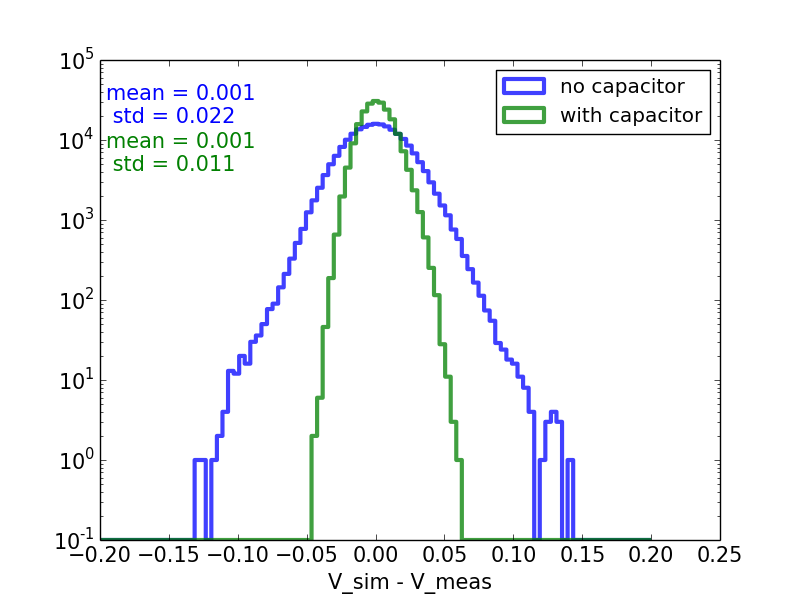
\includegraphics[width=0.49\linewidth]{residualpd.png}}
  \caption{}
  \label{fig:m2ex}
\end{figure}


\newpage
\paragraph{convolution with fixed parameters (method 3)}
For the first  method we had found that depending  on the waveform the
result for  the linear transformation parameters would  vary, which is
not really  meaningful.  We implemented  a third method which  is very
similar to the first one except  that we fix the DC caracterisitcs and
then we  fit the best $\tau$.   We use the relation  found between the
average the RF  waveform in dBm and the average  of the power detector
waveform (see  fig~\ref{fig:pdcarac}) and produce  the convolution the
same way as describe before.  The  decay time constant we find in this
case is  slightly different, we find  $\rm \tau_{capa} =  41.5 ns$ and
$\rm  \tau_{capa}   =  6.3  ns$.    The  results  are  shown   in  the
fig.~\ref{fig:m3ex}
\begin{figure}[!ht]
  \centering
  \hspace*{-3ex}
  \subfigure{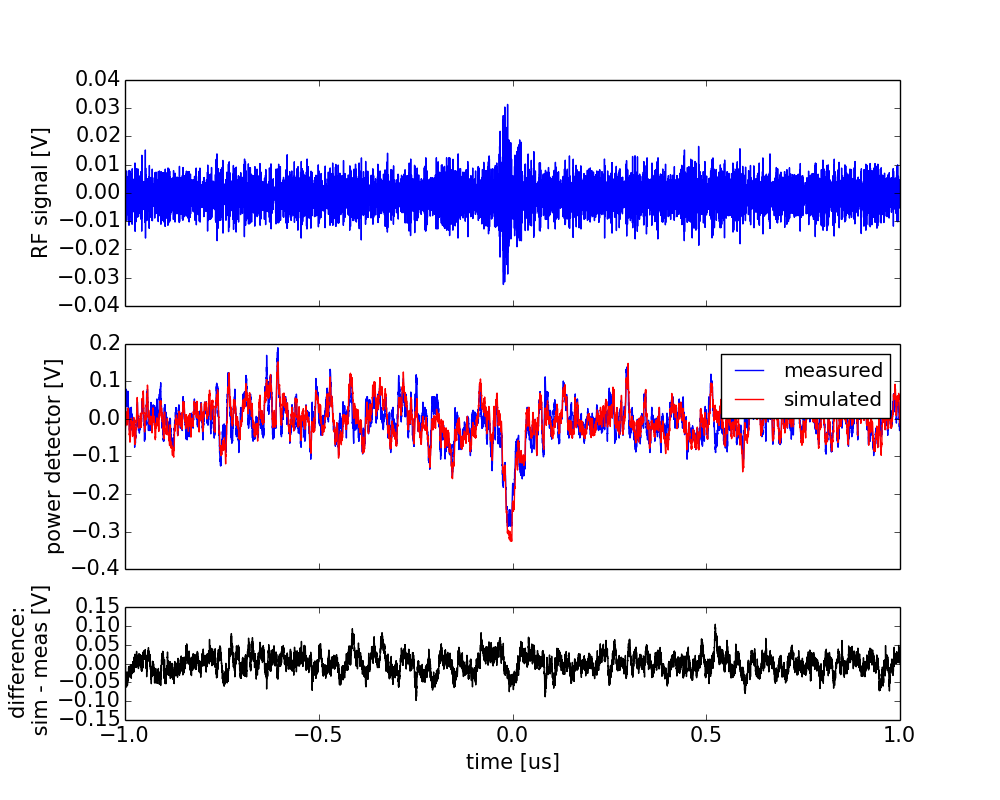
\includegraphics[width=0.49\linewidth]{nocapa_method3.png}}
  \subfigure{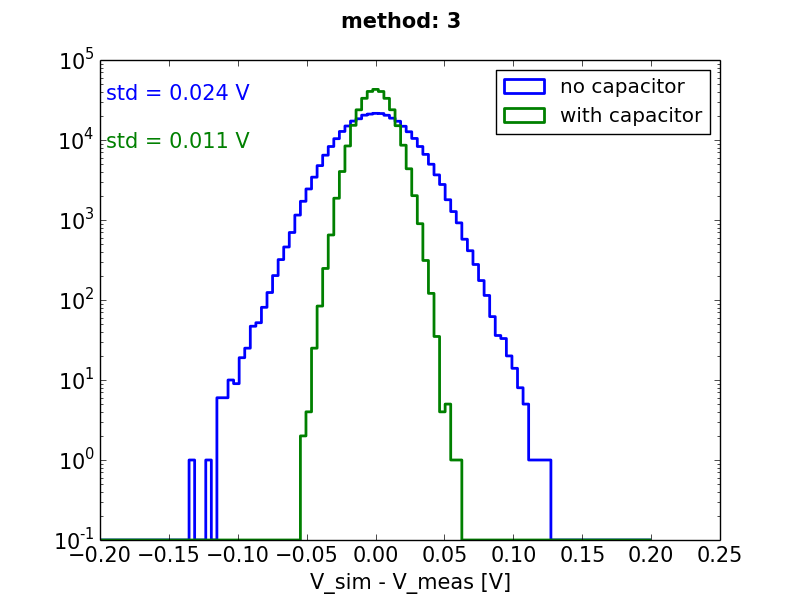
\includegraphics[width=0.49\linewidth]{res_method3.png}}
%  \subfigure{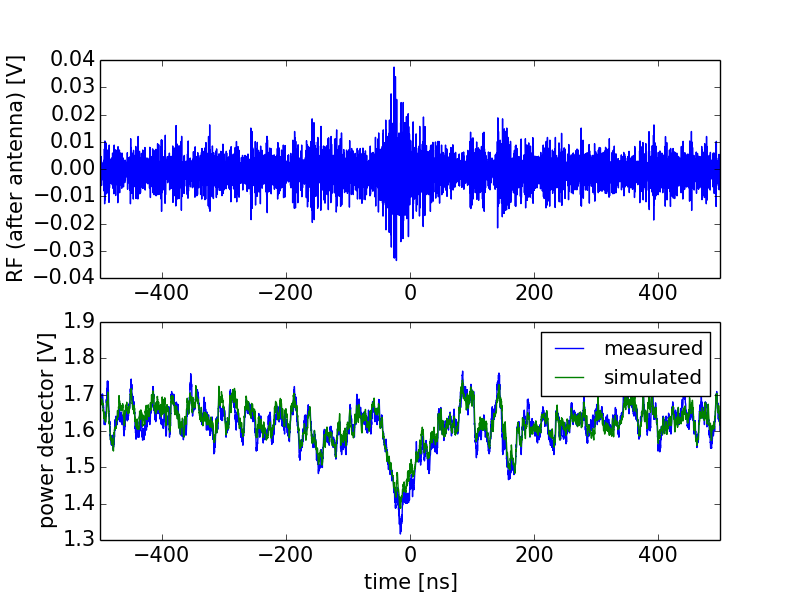
\includegraphics[width=0.49\linewidth]{examplepowerdetsim.png}}
%  \subfigure{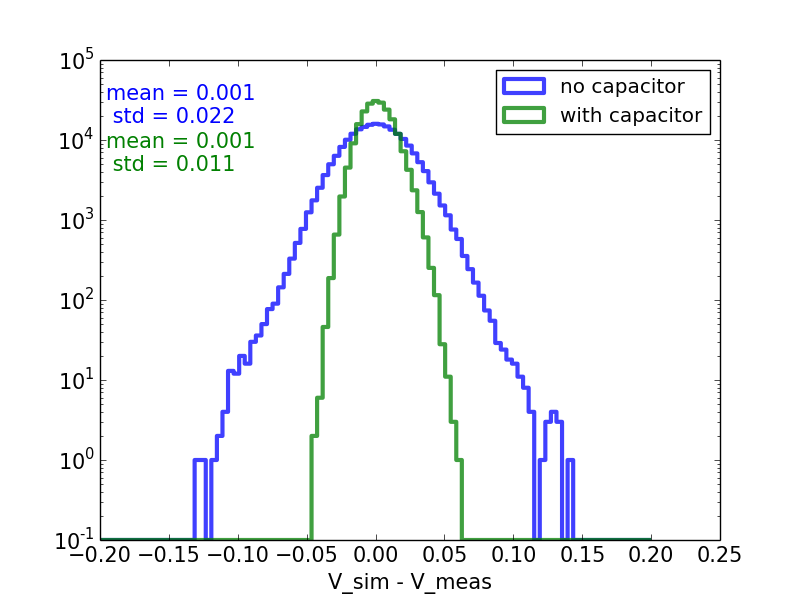
\includegraphics[width=0.49\linewidth]{residualpd.png}}
  \caption{}
  \label{fig:m3ex}
\end{figure}
The residuals  found with  this method  are as good  as for  the first
method.

\clearpage
\subsection{easier board}
This stage is  an amplification of the power  detector signal in order
to choose the dynamic range we want  to keep at the final stage. It is
performed with an amplifier and adjustable voltage offset.  Up to now,
this step  was simulated  with a linear  transformation.  We  will see
that  we  need to  account  for the  dependence  in  frequency of  the
amplifier.\\To determine the characteristics of this stage, we had set
up an experiment with a  C-band antenna followed by the power detector
and an EASIER board.  The signal was recorded after the power detector
and after the board  (see figure~\ref{fig:exampleboard}).  \\ First we
look  at the characteristics  $\rm <V_{board}>  = f(<V_{PD}>)$  of the
mean  value  of   the  waveforms  (see  figure~\ref{fig:carac}  left).
However,  when we  look at  the characteristics  for $\rm  V_{board} =
f(V_{PD})$  we obtain a  different result  (see figure~\ref{fig:carac}
right).   That  means  that  the  response for  the  DC  component  is
different  from  the  higher  frequencies, or  equivalently  that  the
amplifier gain is not flat in frequency.
\begin{figure}[!ht]
  \centering
  \hspace*{-3ex}
  \subfigure{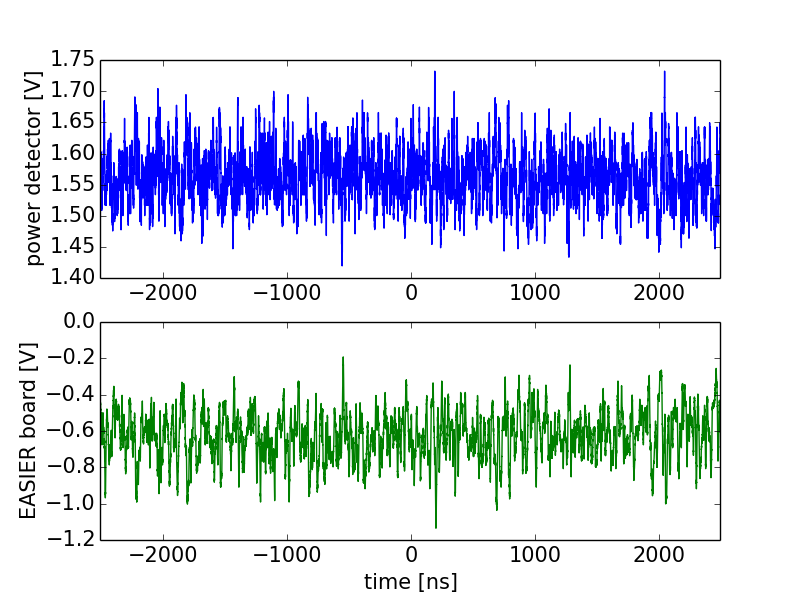
\includegraphics[width=0.60\linewidth]{exampleeasierboard.png}}
  \caption{example  of waveform  after  the power  detector (top)  and
    aftern the EASIER board (bottom) }
  \label{fig:exampleboard}
\end{figure}

\begin{figure}[!ht]
  \centering
  \hspace*{-3ex}
  \subfigure{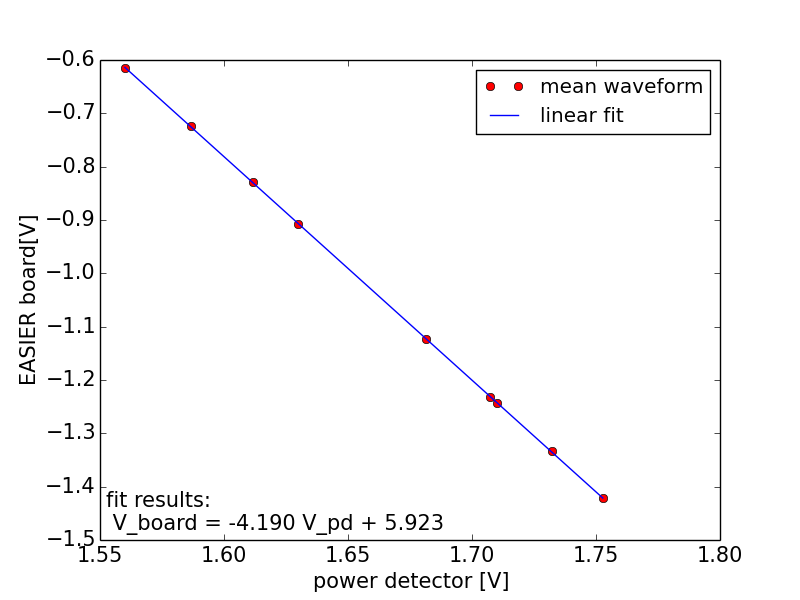
\includegraphics[width=0.45\linewidth]{boardcaracDC.png}}
  \subfigure{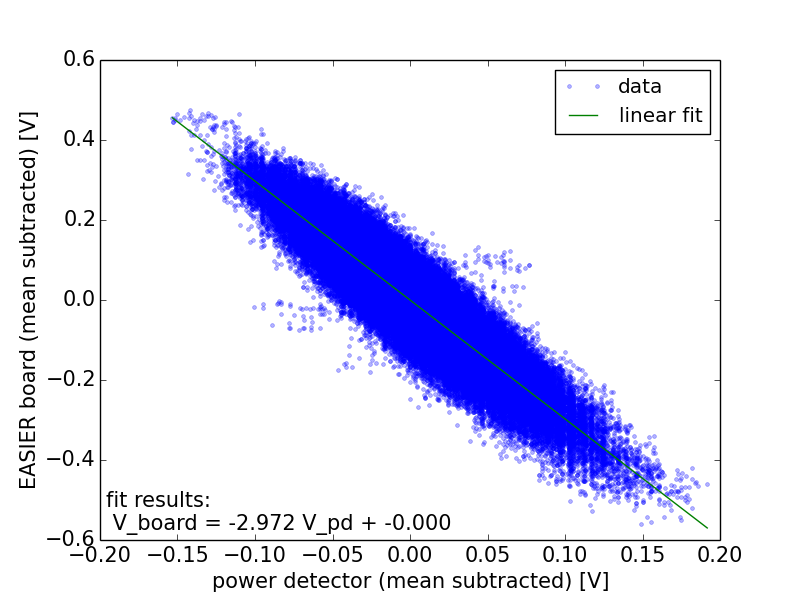
\includegraphics[width=0.45\linewidth]{boardcaracHF.png}}
  \caption{caracteristics of  the easier board for the  average of the
    waveform (left) or for all the points when the baseline is removed
    (right)}
  \label{fig:carac}
\end{figure}

We determine the  response in frequency of the  board taking the ratio
of the FFT of the waveforms.  An example of the FFT of one waveform is
shown in figure~\ref{fig:examplefft}.
\begin{figure}[!ht]
  \centering
  \hspace*{-3ex}
  \subfigure{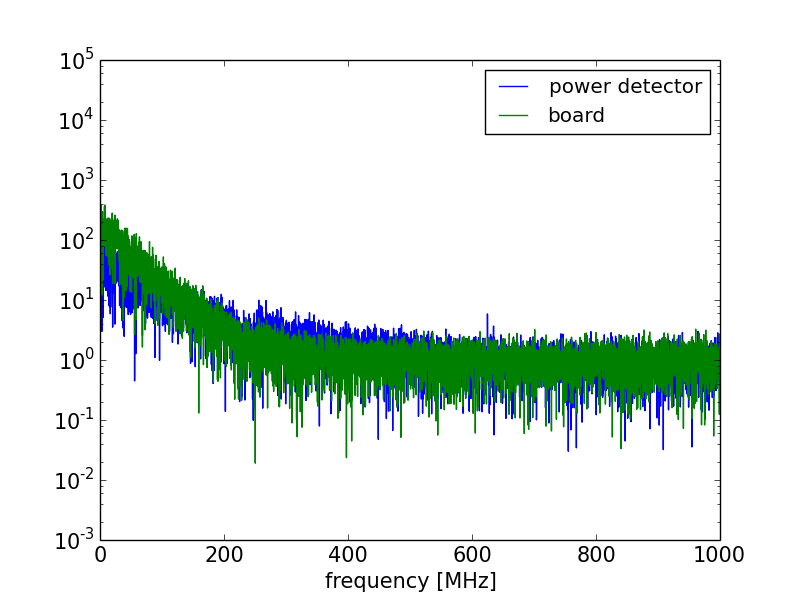
\includegraphics[width=0.32\linewidth]{fftexspec.png}}
  \subfigure{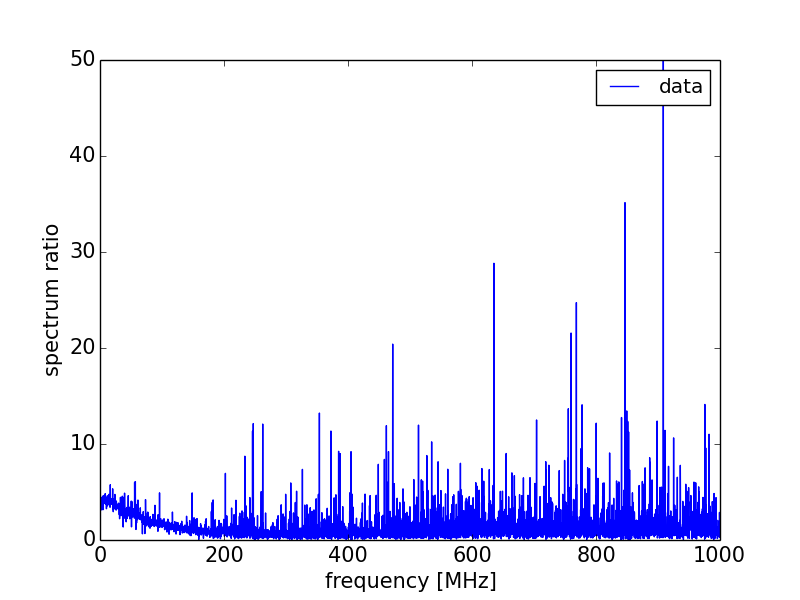
\includegraphics[width=0.32\linewidth]{fftexratio.png}}
  \subfigure{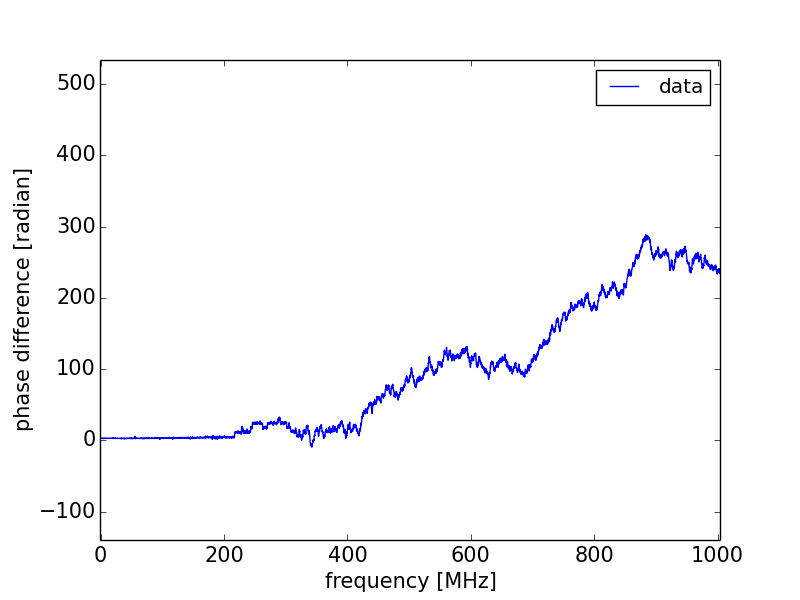
\includegraphics[width=0.32\linewidth]{fftexphase.png}}
  \caption{Left:  example of  spectra of  the power  detector  and the
    easier board. Middle: the ratio of the spectra on the left. Right:
    phase difference between the two fft.}
  \label{fig:examplefft}
\end{figure}
We see that  it is really noisy,  that's because it is FFT  of noise !
Most of  the power is in the  first 200MHz. For the  spectrum we could
average  over   multiple  spectra,   for  the  phase   we  encountered
difficulties to average  it due to phase jumps.  So  we fit an average
spectrum and fit only one phase.  Then to obtain the board signal from
the power detector the first step is to make the non DC frequencies go
through the response we found and then add the correct offset with the
$\rm <V_{board}>  = f(<V_{PD}>)$ characteristic.  \\  The fitted curve
shown in red on figure~\ref{fig:fitboard} are:
\begin{samepage}
  \begin{itemize}
  \item spectrum:  $\rm s = a\cdot  e^{-\frac{(x-\mu)^2}{2\sigma^2}} + k
    $\\ with a =  3.86, $\rm \mu = -40$ , $\rm \sigma =  75.1$ , k = 1.0
    and x is the frequency in MHz
  \item phase: $\rm p = ax^2 + bx + c $ \\ with a = 4.8 $\rm 10^{-5}$, b
    = -1.1 $\rm 10^{-3}$, c = 2.97
  \end{itemize}
\end{samepage}

\begin{figure}[!ht]
  \centering
  \hspace*{-3ex}
  \subfigure{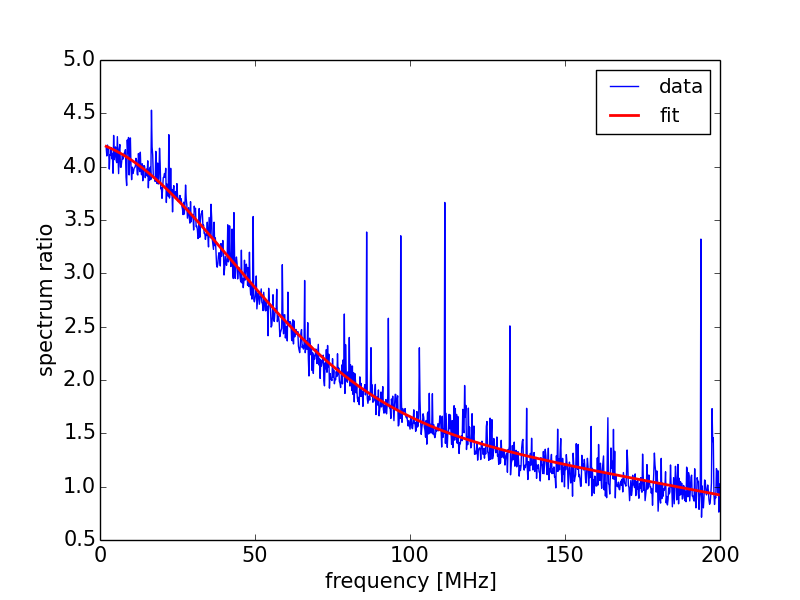
\includegraphics[width=0.45\linewidth]{fitspecboard.png}}
  \subfigure{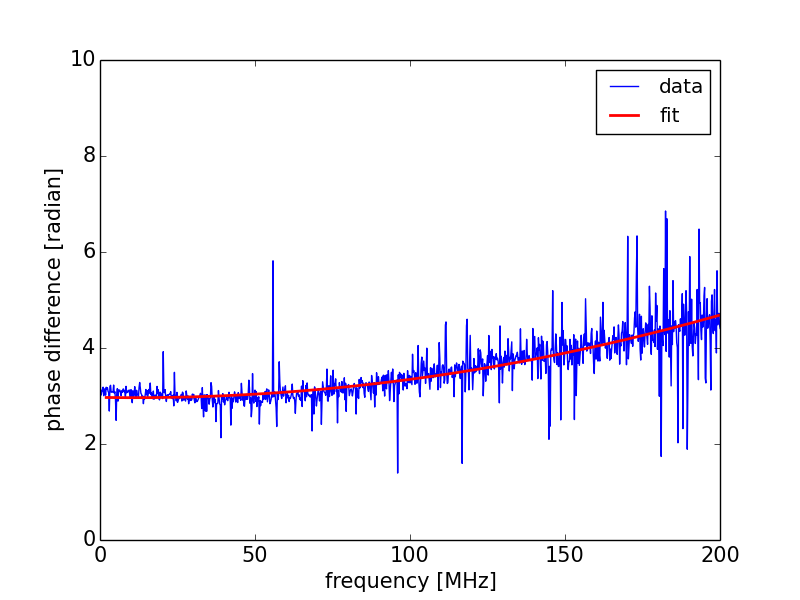
\includegraphics[width=0.45\linewidth]{fitphaseboard.png}}
  \caption{Fit of the board response (spectrum on the left, phase on the left), function and parameters are given in the text}
  \label{fig:fitboard}
\end{figure}

Now we  can look at the  comparison between the old  simulation with a
constant gain and  the new method with a  frequency dependent gain. An
example of waveforms (measured, simulated  with old and new method) is
shown in  figure~\ref{fig:simboard} left and  the difference histogram
is given on the right.
\begin{figure}[!ht]
  \centering
  \hspace*{-3ex}
  \subfigure{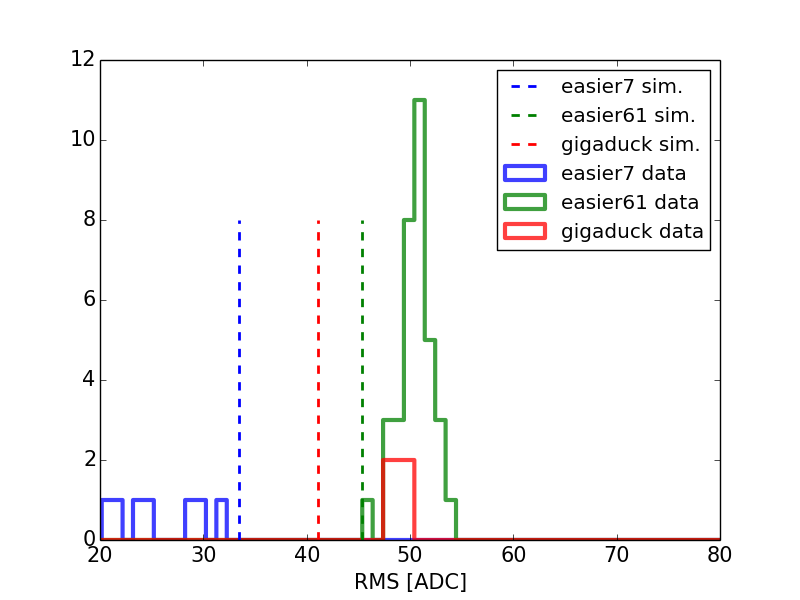
\includegraphics[width=0.33\linewidth]{datasimrmsdist.png}}
  \subfigure{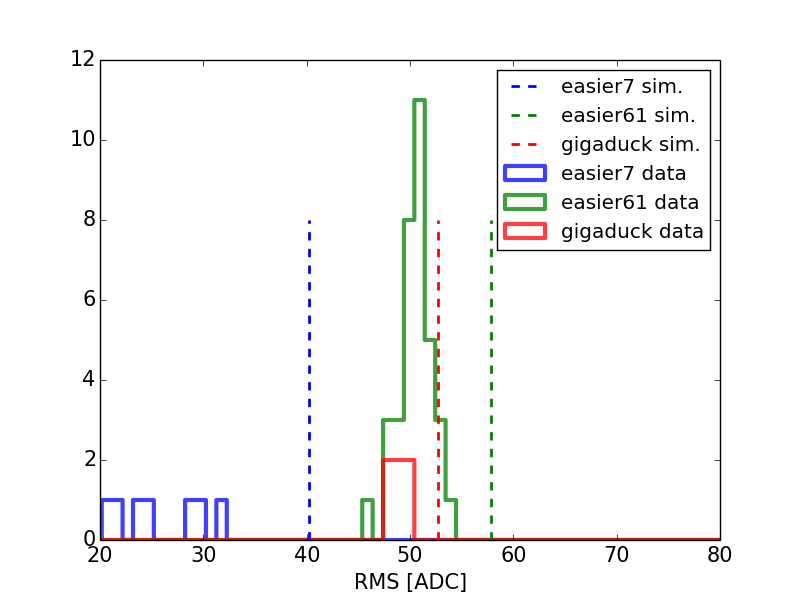
\includegraphics[width=0.33\linewidth]{m2_datasimrmsdist.png}}
  \subfigure{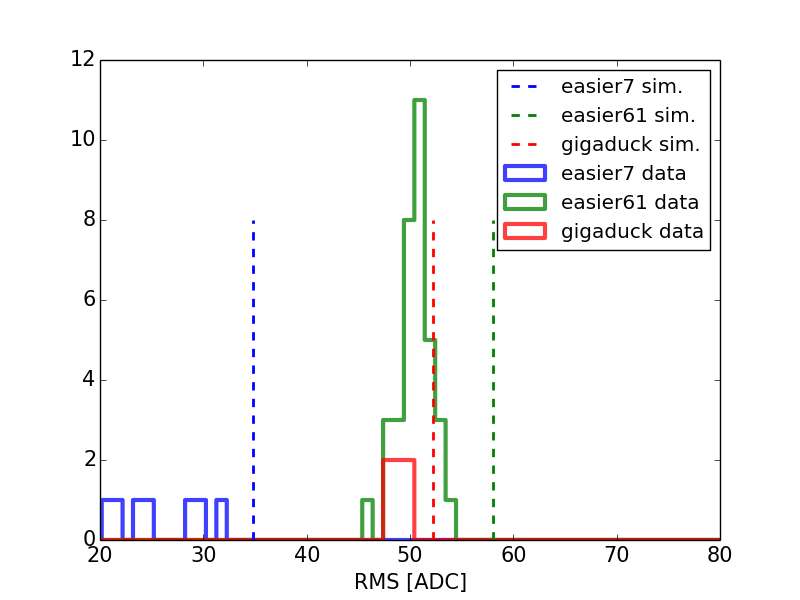
\includegraphics[width=0.33\linewidth]{m3_datasimrmsdist.png}}
  \caption{comparison of the measured distribution of amplitude and the simulated one.}
  \label{fig:datatrace}
\end{figure}


\begin{figure}[!ht]
  \centering
  \hspace*{-3ex}
  \subfigure{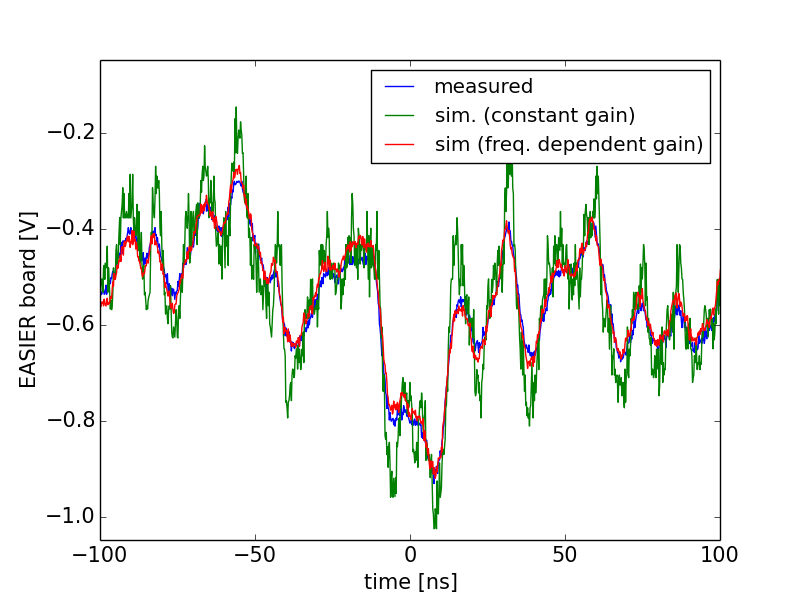
\includegraphics[width=0.45\linewidth]{examplesimboard.png}}
  \subfigure{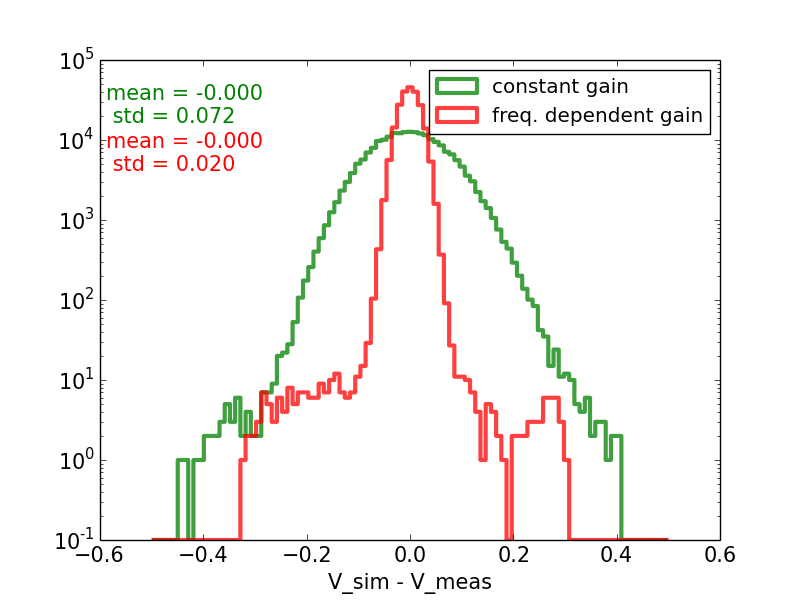
\includegraphics[width=0.45\linewidth]{residualboard.png}}
  \caption{left:waveforms  (measured  and  simulated), right:  voltage
    difference of around 20 waveforms}
  \label{fig:simboard}
\end{figure}

\newpage
\subsection{SD front end}
This is  the last piece  of the electronics  chain. We don't  have any
data to look  at its response.  From the Auger  technical report it is
composed of a  low pass filter ($\rm f_{cut}  = 20~MHz$).  We simulate
it with a butterworth filter of 4th order.


